% !TEX TS-program = XeTeX
% !TEX encoding = UTF-8 Unicode
% !TEX spellcheck = gr-GR

\documentclass[12pt]{turabian-researchpaper}
\usepackage{fontspec}
\usepackage{polyglossia}
\usepackage{setspace}
\usepackage{ragged2e}
\usepackage{geometry}
\usepackage{graphicx}
\usepackage{titlesec}
\usepackage{booktabs}
\usepackage{array}
\usepackage{amsmath}
\usepackage{paralist}
\usepackage{fancyhdr}
\usepackage{multicol}
\usepackage{pagecolor}
\usepackage{enumitem}
\usepackage{svg}
\usepackage{xcolor}
\usepackage[hidelinks]{hyperref}

\geometry{a4paper}
\geometry{margin=2.4cm}
\setmainfont{GFS Didot}
\setdefaultlanguage{greek}

\setstretch{1.2}
\justifying

\definecolor{calm white}{HTML}{F3F3F3}
\definecolor{dark grey}{HTML}{303030}
% \pagecolor{calm white}
\color{dark grey}

\graphicspath{ {.} }

\titleformat{\section}
       {\normalfont\fontsize{15}{18}\bfseries}
       {\thesection}
       {1em}
       {}
\titleformat{\subsection}
       {\normalfont\fontsize{12}{15}\bfseries\itshape}
       {\thesubsection}
       {1em}
       {}

\title{Εξέταση Θεωρίας}
% \subtitle{Ιούνιος 2021}
\author{Ζαμάγιας Μιχαήλ Ανάργυρος -- ΤΠ5000}
\course{Διαχείρηση Έργων Πληροφορικής}
\date{\today}

\begin{document}

\begin{titlepage}
    \maketitle
\end{titlepage}

\tableofcontents

\newpage

\section{Θέμα 1}

\subsection{1. Τι είναι διαχείριση ενός έργου;}

Η ικανότητα να γίνει διαχείριση ενός προσωρινού προβλήματος, ώστε να δημιουργηθεί ένα μοναδικό προϊόν ή υπηρεσία – μέσα στον χρόνο του και στα πλαίσια του προϋπολογισμού.

\subsection{3. Περιγράψτε σύντομα τι είναι η ανάλυση δικτύου στη Διαχείριση Έργων και ποιες τεχνικές γνωρίζετε που χρησιμοποιούνται για την ανάλυση ενός δικτύου. Ποιες είναι οι κύριες διαφορές τους;}

Η Δομή Ανάλυσης Εργασιών είναι μια ιεραρχική ανάλυση της απαιτούμενης εργασίας σε πακέτα εργασίας (work packages) και δραστηριότητες (tasks), προσανατολισμένη στα παραδοτέα (deliverables). Δύο τεχνικές χρησιμοποιούνται για την ανάλυση ενός δικτύου, η "από κάτω προς τα πάνω"/"bottom-up" και η "από επάνω προς τα κάτω"/"top-down".

Στην "top-down" τεχνική:
\begin{itemize}
    \item Η εργασία γίνεται σε ένα ήδη δημιουργημένο σχέδιο έργου, με τις κύριες δραστηριότητες να είναι ήδη γνωστές.
    \item Κάθε κύρια δραστηριότητα υποδιαιρήται σε συγκεκριμένες υποδραστηριότητες και κάθε υποδραστηριότητα αναδιατάσσεται σε υπουποδραστηριότητες. Έτσι, δημιουργείται μια ιεραρχική δομή δέντρου, η οποία είναι χαρακτηριστική για την ΔΑΕ (WBS).
\end{itemize}

Στην "bottom-up" τεχνική:
\begin{itemize}
    \item Αν δεν υπάρχει ακόμη σαφές σχέδιο έργου, είναι επίσης πιθανό να ξεκινήσουμε από το κάτω μέρος και να υπολογίσουμε ποιες μεμονωμένες / επιμέρους δραστηριότητες θα πρέπει να εκτελεστούν.
    \item Μετά οι συναφείς δραστηριότητες μπορούν να ομαδοποιηθούν σε υψηλότερο επίπεδο, κλπ
    \item Με τον τρόπο αυτό δημιουργούμε την ιεραρχική δομή δέντρου, που ομαδοποιείται όπως ανεβαίνουμε προς τα πάνω σε διάφορες υπο-δραστηριότητες κι ενότητες εργασίας.
\end{itemize}


\subsection{4. H τεχνική αξιολόγησης και αναθεώρησης έργου PERT (Program Evaluation and Review Technique) είναι:}
Μία μέθοδος εκτίμησης χρόνου υλοποίησης ενός έργου, λαμβάνοντας υπόψη τις απαισιόδοξες, τις αισιόδοξες και τις πλέον πιθανές εκτιμήσεις αναφορικά με τον χρόνο υλοποίησης των δραστηριοτήτων ενός έργου.

\subsubsection{Τι ονομάζουμε «συμπίεση ενός έργου (project crashing)»;}

Η «συμπίεση ενός έργου (project crashing)» είναι μια μέθοδος για τη μείωση της χρονικής διάρκειας του έργου, μειώνοντας την διάρκεια μερικών κρίμιμων δραστηριοτήτων του έργου σε λιγότερο από τον αρχικά προγραμματισμένο τους χρόνο.

\subsubsection{Ποια κόστη εμπλέκονται στην συμπίεση ενός έργου;}

Δύο είδη κόστους εμπλέκονται στην συμπίεση ενός έργου, τα άμεσα και τα έμμεσα κόστη. Άμεσα κόστη, π.χ.: μισθοί, κόστος πρώτων υλών και χρήσης μηχανημάτων, κτλ. Έμεσσα κόστη, π.χ.: γενικά λειτουργικά έξοδα διεύθυνσης και διαχείρισης έργου, ασφάλιστρα, φόροι, τόπο, κτλ.

\section{Θέμα 2}

\subsubsection{1. Περιγράψετε σε τι αναφέρεται η PRINCE2 με τους όρους \textit{Διαχείρηση κατά φάσεις} και \textit{Διαχείρηση κατ' εξαίρεση}.}

\subsubsection{Διαχείρηση κατά φάσεις}
Ένα έργο χωρίζεται σε διάφορα στάδια διαχείρισης. Κάθε έργο πρέπει να έχει ένα στάδιο που ονομάζεται το στάδιο έναρξης, όπου αναπτύσσονται μια λεπτομερής επιχειρηματική υπόθεση, σχέδιο έργου και στρατηγικές για τη διαχείριση κινδύνων, ζητημάτων, αλλαγών, ποιότητας, προϊόντων και επικοινωνιών. Στη συνέχεια, υπάρχουν ένα ή περισσότερα στάδια «παράδοσης» τα οποία είναι στάδια διαχείρισης όπου αναπτύσσονται εξειδικευμένα προϊόντα. Πριν προχωρήσουμε στο επόμενο στάδιο, η ενημερωμένη επιχειρηματική υπόθεση επανεξετάζεται για να προσδιοριστεί εάν το έργο εξακολουθεί να έχει επιχειρησιακή αιτιολόγηση. Εάν το κάνει, τότε το έργο μπορεί να προχωρήσει στο επόμενο στάδιο. Όπως αναφέρθηκε προηγουμένως, εάν δεν υπάρχει πλέον αιτιολόγηση επιχείρησης, το έργο πρέπει να κλείσει. Επομένως, στο PRINCE2, ένα όριο σταδίου διαχείρισης σχηματίζει ένα σημείο απόφασης «Go / No go» και αποτελεί τον κύριο έλεγχο για το Project Board, το οποίο είναι ο κύριος υπεύθυνος λήψης αποφάσεων για ένα έργο.

\subsubsection{Διαχείριση κατ' εξαίρεση}
Τα άτομα στο Διοικητικό Συμβούλιο του Έργου θεωρείται ότι είναι ανώτερα από εκείνα που έχουν λιγότερο χρόνο στην διαχείριση του έργου. Η καθημερινή διαχείριση είναι ευθύνη του διαχειριστή του έργου. Το Διοικητικό Συμβούλιο του Έργου επομένως αναθέτει την καθημερινή διαχείριση για ένα στάδιο στον διαχειριστή του έργου εντός συμφωνημένων «ανοχών» για τους στόχους του χρόνου, του κόστους, του κινδύνου και του πεδίου εφαρμογής. Με την προϋπόθεση ότι ο διαχειριστής του έργου είναι βέβαιος ότι μπορεί να παραδώσει το σχέδιο σκηνής μέσα σε αυτές τις συμφωνημένες ανοχές, τότε μπορεί να λάβει διορθωτικά μέτρα για να επαναφέρει τα πράγματα σε τροχιά, αν τα πράγματα καθυστερούν να υπερβούν τον προϋπολογισμό.

Εάν, ωστόσο, ο διαχειριστής του έργου δεν μπορεί να παραδώσει το σχέδιο σκηνής εντός αυτών των συμφωνημένων ανοχών σταδίου, τότε αυτό είναι γνωστό ως «εξαίρεση» στο PRINCE2 και αυτό πρέπει να διαβιβαστεί στο συμβούλιο του έργου για απόφαση. Επομένως, αυτή είναι μια πολύ αποτελεσματική χρήση του ανώτερου διοικητικού χρόνου και σημαίνει ότι το συμβούλιο του έργου συμμετέχει στη λήψη αποφάσεων μόνο όταν και όταν χρειάζεται. (Φυσικά εξακολουθούν να συμμετέχουν στη λήψη των βασικών αποφάσεων «Go / No go» στο τέλος κάθε σταδίου).

\section{Θέμα 3}
\subsection{1. Ποια είναι η κρίσιμη διαδρομή και ποιος ο χρόνος περάτωσης του έργου;}
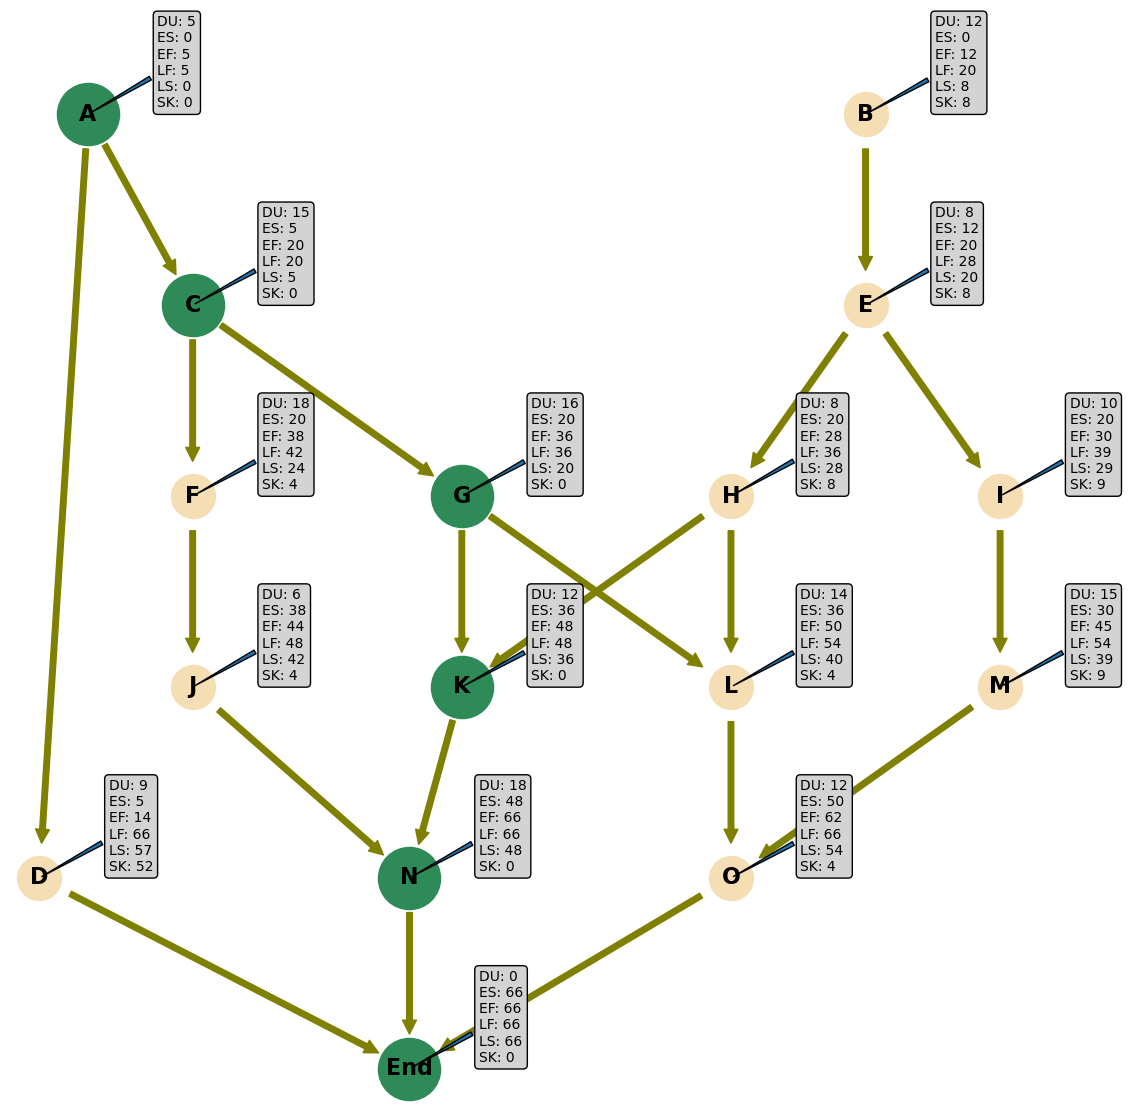
\includegraphics[scale=0.33]{cpm_0.png}
\begin{table}[]
    \centering
    \begin{tabular}{|ll|}
        \hline
        Αριθμός & Όνομα \\ \hline
        101     & A     \\
        102     & B     \\
        201     & C     \\
        202     & D     \\
        203     & E     \\
        301     & F     \\
        302     & G     \\
        303     & H     \\
        304     & I     \\
        401     & J     \\
        402     & K     \\
        403     & L     \\
        404     & M     \\
        501     & N     \\
        502     & O     \\ \hline
    \end{tabular}
\end{table}

Κρίσιμη διαδρομή: $101 (A) \rightarrow  201 (C) \rightarrow 302(G) \rightarrow 402 (K) \rightarrow 501 (N) \rightarrow End$

Χρόνος περάτωσης: $66$ ημέρες

\subsection{2. Αν η δραστηριότητα 203 καθυστερήσει κατά 7 ημέρες πώς θα επηρεαστεί ο χρόνος υλοποίησης του έργου και γιατί;}

Αν η δραστηριότητα 203 καθυστερήσει κατά 7 ημέρες, η δραστηριότητα 502 θα καθυστηρήσει 2 ημέρες, αλλά ο χρόνος υλοποίησης του έργου δεν θα επηρεαστεί.

\subsection{3. Αν η δραστηριότητα 301 απαιτήσει 16 ημέρες αντί για 18 πώς θα επηρεαστεί ο χρόνος υλοποίησης του έργου και γιατί;}

Δεν θα επηρεαστεί ο χρονος υλοποίησης του εργου, καθώς η 301 δεν αποτελεί κρίσιμη δραστηριότητα (αφού έχει $SK = 4$).

\section{Θέμα 4}

\subsection*{1. Ποιος είναι ο αναμενόμενος χρόνος ολοκλήρωσης του έργου;}
Αναμενόμενος χρονος: $20$ εβδομάδες

\subsection{2. Ποια η πιθανότητα το έργο να ολοκληρωθεί μια εβδομάδα πιο πριν από ότι αναμένεται;}
Πιθανότητα: $31.56\%$

\subsection{3. Ποια η πιθανότητα το έργο να μην ολοκληρωθεί εντός $22$ εβδομάδων;}
Πιθανότητα: $16.6\%$

\subsection{4. Ποιος είναι ο αναμενόμενος χρόνος ολοκλήρωσης του έργου; Αν θέλουμε να έχουμε πιθανότητα μόνο $10\%$ να αποτύχουμε στον προγραμματισμό των ενεργειών μας, τότε πόσο εκτιμάτε πως θα διαρκέσει το έργο;}
Χρόνος: $22.6$ εβδομάδες

\subsection*{Πράξεις}

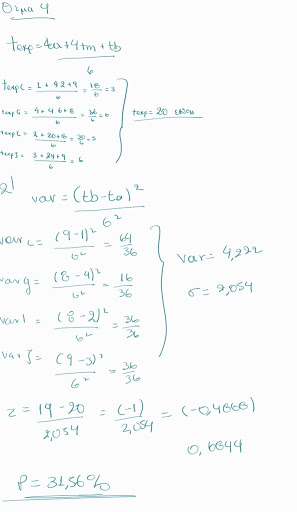
\includegraphics[scale=1.2]{4_i.jpg}

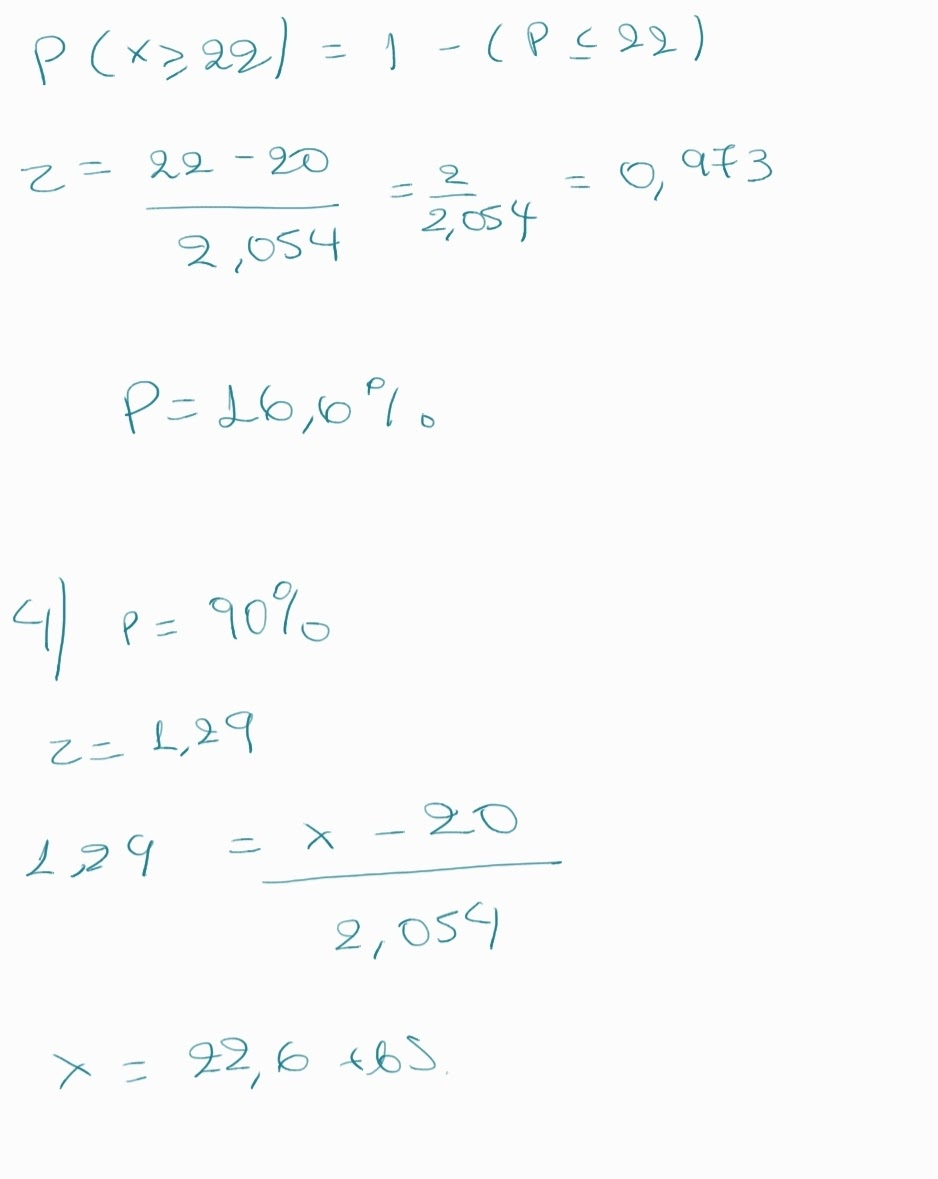
\includegraphics[scale=0.42]{4_ii.jpg}

\end{document}
